\chapter{Aritmetica binaria e logica booleana}

\section{Introduzione}
Partiamo con il dire che tutti i calcolatori moderni possono essere schematizzati semplicemente
tramite il cosiddetto \textbf{modello Von Neumann} in cui abbiamo tre componenti principali:
\textbf{memoria}, \textbf{processore} e canali di \textbf{I/O}.

\begin{center}
	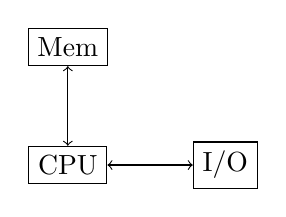
\begin{tikzpicture}
		\node[draw] (mem) at (0, 0) {Mem};
		\node[draw] (cpu) at (0, -1.5) {CPU};
		\node[draw] (io) at (2, -1.5) {I/O};

		\draw[<->] (mem) -- (cpu);
		\draw[<->] (cpu) -- (io);
	\end{tikzpicture}
\end{center}

Come possiamo vedere dalla figura i collegamenti tra le varie entità sono bidirezionali. Il
processore (ma anche la memoria) è collegato ai canali di I/O e il collegamento che c'è tra memoria
e processore è chiamato \textbf{Von Neumann bottleneck}. Quello che accade tra memoria e processore
è, grosso modo, quello che viene descritto dal seguente pseudocodice.

\begin{minted}{c}
while (true) {
	istr = M[PC]
	decode(istr)
	res = exec(istr)
	update(PC)
	writeback(res)
	interrupt_handling()
}
\end{minted}

In pratica viene estratta dalla memoria l'istruzione puntata da un \textbf{Program Counter}, la
si decodifica e la si esegue. In seguito il Program Counter viene aggiornato e i risultati vengono
consolidati nei registri della CPU oppure in memoria.

